\documentclass[11pt,a4paper]{article}

% === Encodage et langue ===
\usepackage[utf8]{inputenc}
\usepackage[T1]{fontenc}
% babel french non disponible — on gère manuellement
\usepackage{csquotes}

% === Mise en page ===
\usepackage[margin=2.2cm]{geometry}
\usepackage{fancyhdr}
\usepackage{lastpage}

% === Mathématiques et unités ===
\usepackage{amsmath,amssymb}
\usepackage{siunitx}
\sisetup{
  locale = FR,
  group-separator = {\,},
  output-decimal-marker = {,},
  per-mode = symbol,
}

% === Tableaux ===
\usepackage{booktabs}
\usepackage{multirow}
\usepackage{array}
\usepackage{colortbl}

% === Graphiques et couleurs ===
\usepackage{graphicx}
\usepackage[dvipsnames,table]{xcolor}
\usepackage{tikz}
\usetikzlibrary{arrows.meta,patterns,decorations.pathmorphing,calc}

% === Divers ===
\usepackage{enumitem}
\usepackage{caption}
\usepackage{subcaption}
\usepackage{hyperref}
\hypersetup{
  colorlinks=true,
  linkcolor=NavyBlue,
  citecolor=ForestGreen,
  urlcolor=RoyalBlue,
}

% === En-tête / pied de page ===
\pagestyle{fancy}
\fancyhf{}
\lhead{\small\textsc{Simulation Geant4 --- MiniX X-Ray Tube}}
\rhead{\small Collimateur 3\,mm (Al + Laiton)}
\cfoot{\small Page \thepage/\pageref{LastPage}}
\renewcommand{\headrulewidth}{0.4pt}
\renewcommand{\footrulewidth}{0.2pt}

% === Couleurs personnalisées ===
\definecolor{brass}{RGB}{181,166,66}
\definecolor{aluminium}{RGB}{169,172,182}
\definecolor{graphite}{RGB}{52,73,94}
\definecolor{airblue}{RGB}{52,152,219}
\definecolor{lightgray}{RGB}{245,245,245}

% === Titre ===
\title{%
  \vspace{-1.5cm}
  {\Large\textsc{Simulation Monte Carlo Geant4}}\\[0.3cm]
  {\LARGE\bfseries Statistiques de référence --- Collimateur 3\,mm}\\[0.2cm]
  {\large\itshape 5 millions d'événements primaires}\\[0.3cm]
  {\normalsize Configuration : Al + Laiton + Porte-collimateur Inox\,304}
}
\author{%
  Tube à rayons X Amptek MiniX (\SIrange{1}{50}{\kilo\electronvolt}, cône \ang{60})
}
\date{\today}

\begin{document}
\maketitle
\thispagestyle{fancy}

% ======================================================================
\section{Paramètres de la simulation}
% ======================================================================

\begin{table}[h!]
\centering
\caption{Paramètres du run de référence.}
\label{tab:params}
\begin{tabular}{@{}ll@{}}
\toprule
\textbf{Paramètre} & \textbf{Valeur} \\
\midrule
Code & Geant4 11.03-patch-01 (MT, 21 mars 2025) \\
Primaires générés & \num{5000000} photons $\gamma$ \\
Spectre d'émission & \SIrange{3.5}{50}{\kilo\electronvolt} (anode W) \\
Géométrie d'émission & Cône de demi-angle \ang{60} \\
Collimateur interne & Al ($\varnothing_{\text{int}} = \SI{2.0}{\milli\metre}$, ép.\ \SI{25}{\micro\metre}) \\
Collimateur externe & Laiton ($\varnothing_{\text{int}} = \SI{2.05}{\milli\metre}$, ép.\ \SI{2.1}{\milli\metre}) \\
Porte-collimateur & Inox 304 ($R_{\text{int}} = \SI{3.17}{\milli\metre}$, $R_{\text{ext}} = \SI{5.9}{\milli\metre}$) \\
Plan de scoring & ScorePlane1 à $z = \SI{18}{\milli\metre}$ \\
Cible & Eau (couronnes concentriques, $z = \SIrange{64}{69}{\milli\metre}$) \\
\bottomrule
\end{tabular}
\end{table}

% ======================================================================
\section{Bilan global des photons}
% ======================================================================

Sur les \num{5000000} photons primaires émis dans le cône de \ang{60}, le tableau~\ref{tab:bilan} 
résume le devenir de chaque particule.

\begin{table}[h!]
\centering
\caption{Bilan particule du run de référence.}
\label{tab:bilan}
\begin{tabular}{@{}lr r@{}}
\toprule
\textbf{Catégorie} & \textbf{Nombre} & \textbf{Fraction} \\
\midrule
Primaires générés & \num{5000000} & \SI{100}{\percent} \\
\midrule
Absorbés (effet photoélectrique) & \num{4963401} & \SI{99.27}{\percent} \\
Transmis à ScorePlane1 (outward) & \num{39218} & \SI{0.784}{\percent} \\
Secondaires atteignant ScorePlane1 & 15 & \num{3.0}/M$\gamma$ \\
\midrule
\textit{Contrôle} : phot + transmis & \num{5002619} & $\Delta = -\num{2619}$\footnotemark \\
\bottomrule
\end{tabular}
\end{table}
\footnotetext{Le surplus de $\sim$\num{2600} est dû aux interactions multiples (diffusion + absorption) et aux particules 
entrant puis ressortant de volumes intermédiaires.}

Le taux de transmission de \SI{0.784}{\percent} est cohérent avec l'estimation géométrique fondée 
sur l'angle solide du bore ($R = \SI{1.5}{\milli\metre}$, $z = \SI{17.45}{\milli\metre}$) :
\begin{equation}
  f_{\text{géom}} = \frac{\Omega_{\text{bore}}}{\Omega_{\text{cône}}} 
  = \frac{1 - \cos\!\bigl(\!\arctan\!\frac{R}{z}\bigr)}{1 - \cos(\ang{60})}
  \approx \SI{0.69}{\percent}
  \label{eq:fgeom}
\end{equation}
Le rapport mesuré/prédit $= 0{,}784 / 0{,}69 = 1{,}14$ est proche de l'unité ;
le léger excès s'explique par la transmission à travers 
la paroi mince en aluminium (\SI{25}{\micro\metre}).

% ======================================================================
\section{Absorption par matériau}
% ======================================================================

La figure~\ref{fig:geometry} et le tableau~\ref{tab:absorption} détaillent la répartition
de l'absorption par effet photoélectrique entre les différents matériaux de la géométrie.

\begin{table}[h!]
\centering
\caption{Répartition de l'absorption photoélectrique par matériau (\num{4963401} absorptions).}
\label{tab:absorption}
\small
\begin{tabular}{@{}l S[table-format=7.0] S[table-format=2.2]@{}}
\toprule
\textbf{Matériau} & {\textbf{Absorptions}} & {\textbf{Fraction (\%)}} \\
\midrule
\rowcolor{brass!20} Laiton (Cu--Zn) & 3000877 & 60.46 \\
\rowcolor{aluminium!15} Aluminium & 1637121 & 32.98 \\
Béryllium (fenêtre) & 276383 & 5.57 \\
Air (MyAir) & 27527 & 0.55 \\
Tungstène (anode) & 8006 & 0.16 \\
Al\textsubscript{2}O\textsubscript{3} (tube alumine) & 7009 & 0.14 \\
Inox\,304 (porte-collimateur) & 6478 & 0.13 \\
\midrule
\textbf{Total} & 4963401 & 100.00 \\
\bottomrule
\end{tabular}
\end{table}

Le laiton absorbe à lui seul \SI{60.5}{\percent} des photons, suivi de l'aluminium à \SI{33.0}{\percent}.
Ces deux matériaux constituent le système de collimation actuel et sont responsables de 
\SI{93.4}{\percent} de l'atténuation totale. Le béryllium de la fenêtre de sortie du tube contribue 
à \SI{5.6}{\percent}, essentiellement par absorption des photons de basse énergie ($E < \SI{5}{\kilo\electronvolt}$).
L'inox du porte-collimateur n'absorbe que \SI{0.13}{\percent}, confirmant que le blindage est assuré
quasi-intégralement par le laiton et l'aluminium.

% ======================================================================
\section{Particules secondaires atteignant ScorePlane1}
% ======================================================================

\subsection{Vue d'ensemble}

Sur 5~millions de primaires, seules \textbf{15 particules secondaires} atteignent le plan de scoring,
soit un taux de \num{3.0} par million de $\gamma$ émis. Ce chiffre extrêmement faible confirme 
l'efficacité du blindage en laiton : les fluorescences Cu\,K$\alpha$ et Zn\,K$\alpha$ 
(\SIrange{8}{9}{\kilo\electronvolt}) ont un libre parcours moyen de ${\sim}\SI{5}{\micro\metre}$ 
dans le laiton et sont réabsorbées avant d'atteindre le bore.

\subsection{Détail des 15 secondaires}

Le tableau~\ref{tab:secondaires} résume les caractéristiques de chaque secondaire détecté.

\begin{table}[h!]
\centering
\caption{Caractéristiques des 15 secondaires atteignant ScorePlane1.}
\label{tab:secondaires}
\footnotesize
\begin{tabular}{@{}c c c c c c@{}}
\toprule
\textbf{\#} & \textbf{Particule} & \textbf{Processus} & \textbf{Matériau} & $E_{\text{plan}}$ \textbf{(keV)} & $z_{\text{vertex}}$ \textbf{(mm)} \\
\midrule
0  & $e^-$ & phot  & Air & 6,1  & 18,0 \\
1  & $e^-$ & phot  & Air & 18,7 & 17,7 \\
2  & $e^-$ & phot  & Air & 4,2  & 17,9 \\
3  & $e^-$ & phot  & Al  & 18,8 & 16,5 \\
4  & $e^-$ & phot  & Air & 3,3  & 17,8 \\
5  & $e^-$ & phot  & Air & 1,7  & 17,9 \\
6  & $e^-$ & phot  & Air & 8,7  & 17,9 \\
7  & $e^-$ & phot  & Air & 8,8  & 17,2 \\
8  & $e^-$ & phot  & Air & 6,5  & 19,1 \\
9  & $\gamma$ & eBrem & Al  & 16,6 & 11,4 \\
10 & $e^-$ & phot  & Air & 21,3 & 17,1 \\
11 & $e^-$ & phot  & Air & 3,1  & 18,0 \\
12 & $e^-$ & phot  & Al  & 17,7 & 15,6 \\
13 & $e^-$ & phot  & Air & 2,3  & 17,9 \\
14 & $e^-$ & phot  & Al  & 10,0 & 16,1 \\
\bottomrule
\end{tabular}
\end{table}

\subsection{Analyse par catégorie}

\begin{table}[h!]
\centering
\caption{Répartition des secondaires par type, processus et origine.}
\label{tab:sec_resume}
\begin{tabular}{@{}ll c@{}}
\toprule
\textbf{Critère} & \textbf{Catégorie} & \textbf{Nombre} \\
\midrule
\multirow{2}{*}{Type de particule} 
  & $e^-$ (photoélectron) & 14 \\
  & $\gamma$ (Bremsstrahlung) & 1 \\
\midrule
\multirow{2}{*}{Processus créateur}
  & Effet photoélectrique (\texttt{phot}) & 14 \\
  & Bremsstrahlung (\texttt{eBrem}) & 1 \\
\midrule
\multirow{2}{*}{Matériau d'origine}
  & Air ($z > \SI{16.95}{\milli\metre}$) & 11 \\
  & Aluminium ($z \leq \SI{16.95}{\milli\metre}$) & 4 \\
\midrule
\multirow{2}{*}{Énergie au plan}
  & $E_{\text{moy}}$ & \SI{9.9}{\kilo\electronvolt} \\
  & $E_{\min}$ -- $E_{\max}$ & \SIrange{1.7}{21.3}{\kilo\electronvolt} \\
\bottomrule
\end{tabular}
\end{table}

\paragraph{Interprétation physique.}
Les 11~secondaires créées dans l'air ($z \approx \SIrange{17}{19}{\milli\metre}$) sont des 
\textbf{photoélectrons} arrachés aux molécules de N\textsubscript{2}/O\textsubscript{2} par les 
photons primaires transmis, juste après la sortie du collimateur. Leur énergie cinétique au vertex 
(\SIrange{3.3}{22.7}{\kilo\electronvolt}) correspond à $E_\gamma - E_{\text{liaison}}$ avec 
$E_{\text{liaison}}^{\text{N,O}} \approx \SIrange{0.4}{0.5}{\kilo\electronvolt}$.

Les 4~secondaires originaires de l'aluminium proviennent de la surface interne du tube 
($z \approx \SIrange{11}{16.5}{\milli\metre}$, $r \approx R_{\text{bore}}$). 
Parmi eux, 3~sont des photoélectrons ayant eu suffisamment d'énergie 
pour s'échapper du métal vers le bore, et 1~est un photon de Bremsstrahlung 
émis par un photoélectron énergétique ($E_\gamma = \SI{16.6}{\kilo\electronvolt}$, 
né à $z = \SI{11.4}{\milli\metre}$).

\paragraph{Point clé :} \textbf{Aucune diffusion Compton} n'est observée parmi les secondaires 
détectées. C'est la conséquence directe de la section efficace photoélectrique 
dominante du laiton ($Z = 29$) : 
$\sigma_{\text{phot}} / \sigma_{\text{Compton}} \sim 500$ 
à \SI{10}{\kilo\electronvolt}.

% ======================================================================
\section{Dose déposée dans la cible eau}
% ======================================================================

\begin{table}[h!]
\centering
\caption{Dose par anneau dans la cible eau (couronnes concentriques, épaisseur \SI{5}{\milli\metre}).}
\label{tab:dose}
\begin{tabular}{@{}c S[table-format=2.1] S[table-format=6.1] S[table-format=2.1]@{}}
\toprule
\textbf{Anneau} & {$r_{\min}$--$r_{\max}$ (\si{\milli\metre})} & {$E_{\text{déposée}}$ (\si{\kilo\electronvolt})} & {\textbf{Dose} (\si{\nano\gray})} \\
\midrule
0 & {0--2}  & 19390 & 82.4 \\
1 & {2--4}  & 61001 & 86.4 \\
2 & {4--6}  & 98893 & 84.0 \\
3 & {6--8}  & 5074  & 3.1 \\
4 & {8--10} & {$\sim 0$} & {$\sim 0$} \\
\midrule
\multicolumn{2}{@{}l}{\textbf{Total}} & 184914 & 31.4 \\
\bottomrule
\end{tabular}
\end{table}

La dose est remarquablement uniforme dans les anneaux 0, 1 et 2 
(\SIrange{82}{86}{\nano\gray}), avec une chute abrupte à l'anneau~3 
($\SI{3.1}{\nano\gray}$, facteur $\times 27$ plus faible). 
Cela reflète la taille finie du faisceau collimaté : 
les primaires transmis forment un cône de demi-angle $\sim \ang{4.9}$, 
soit un diamètre de $\sim \SI{9}{\milli\metre}$ à $z = \SI{66.5}{\milli\metre}$ (centre de la cible).

% ======================================================================
\section{Vérification de scaling}
% ======================================================================

\begin{table}[h!]
\centering
\caption{Comparaison des résultats entre le run \num{100000} et le run \num{5000000} événements.}
\label{tab:scaling}
\small
\begin{tabular}{@{}l S[table-format=7.0] S[table-format=7.0] c c@{}}
\toprule
\textbf{Grandeur} & {\textbf{100k evt}} & {\textbf{5M evt}} & \textbf{Ratio} & \textbf{Attendu} \\
\midrule
Primaires     & 100000 & 5000000 & $\times 50{,}0$ & $\times 50$ \\
Transmis      & 730    & 39218  & $\times 53{,}7$ & $\times 50$ \\
Taux transm.  & \multicolumn{1}{c}{\SI{0.73}{\percent}} & \multicolumn{1}{c}{\SI{0.78}{\percent}} & --- & $=$ \\
Secondaires   & 0      & 15     & $\infty$ & --- \\
\bottomrule
\end{tabular}
\end{table}

Le scaling est satisfaisant ($\times 53{,}7$ au lieu de $\times 50$, soit $+\SI{7}{\percent}$), 
la légère déviation étant compatible avec les fluctuations statistiques 
($\sigma_{\text{rel}} \approx 1/\sqrt{730} \approx \SI{3.7}{\percent}$).

% ======================================================================
\section{Schéma de la géométrie de référence}
% ======================================================================

\begin{figure}[h!]
\centering
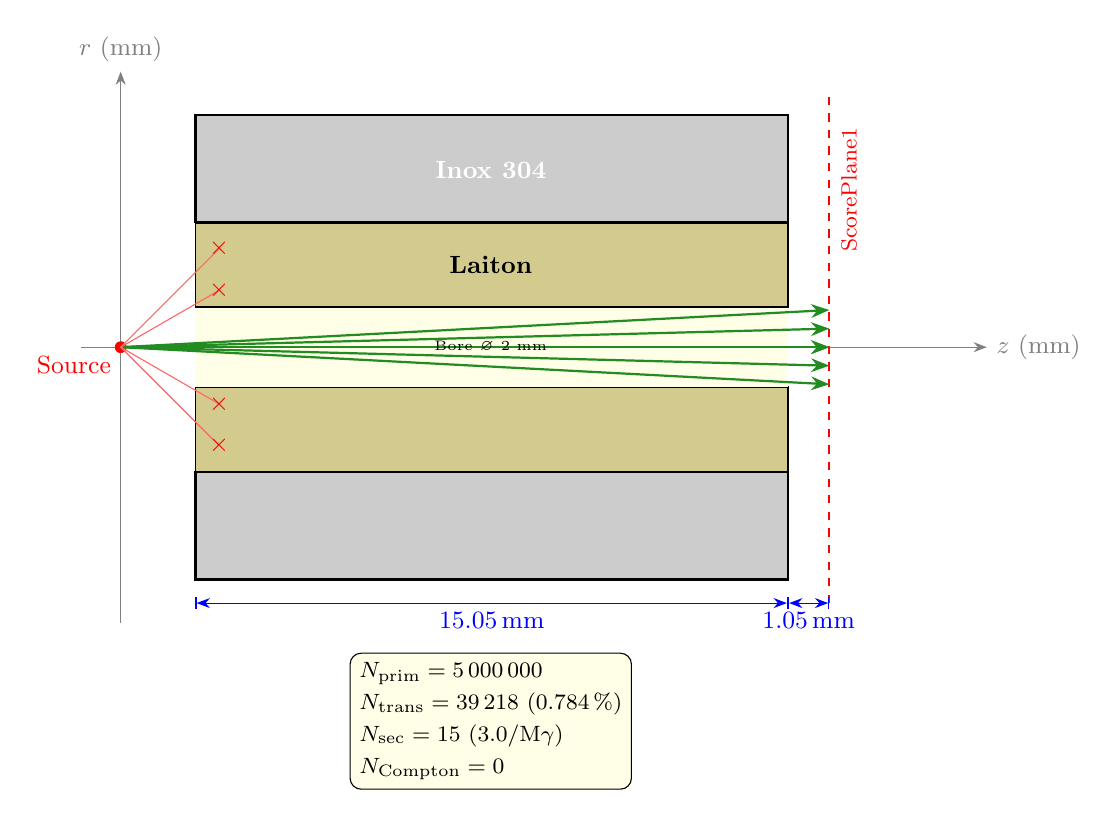
\begin{tikzpicture}[scale=0.50, >=Stealth, every node/.style={font=\small}]
  % Axes
  \draw[->,gray,thin] (-1,0) -- (22,0) node[right] {$z$ (mm)};
  \draw[->,gray,thin] (0,-7) -- (0,7) node[above] {$r$ (mm)};
  
  % Porte-collimateur (Inox 304)
  \foreach \s in {1,-1}{
    \fill[gray!40,draw=black,thick] (1.9,\s*3.17) rectangle (16.95,\s*5.9);
    % Laiton
    \fill[brass!60,draw=black] (1.9,\s*1.024) rectangle (16.95,\s*3.15);
    % Aluminium
    \fill[aluminium!50,draw=black,thin] (1.9,\s*0.999) rectangle (16.95,\s*1.024);
  }
  
  % Bore (air)
  \fill[yellow!10] (1.9,-0.999) rectangle (16.95,0.999);
  
  % Source
  \fill[red] (0,0) circle (0.15);
  \node[below left,red] at (0,0) {Source};
  
  % Scoring plane
  \draw[red,dashed,thick] (18,-6.5) -- (18,6.5);
  \node[red,rotate=90] at (18.5,4) {\footnotesize ScorePlane1};
  
  % Transmitted rays
  \foreach \a in {0,1.5,3}{
    \draw[ForestGreen,thick,->] (0,0) -- ({18},{18*tan(\a)});
    \draw[ForestGreen,thick,->] (0,0) -- ({18},{-18*tan(\a)});
  }
  
  % Absorbed rays
  \foreach \a in {15,30,45}{
    \pgfmathsetmacro{\zhit}{2.5}
    \pgfmathsetmacro{\rhit}{\zhit*tan(\a)}
    \ifdim\rhit pt>1.0pt
      \draw[red!60,thin] (0,0) -- (\zhit,\rhit);
      \node[red] at (\zhit,\rhit) {$\times$};
      \draw[red!60,thin] (0,0) -- (\zhit,-\rhit);
      \node[red] at (\zhit,-\rhit) {$\times$};
    \fi
  }
  
  % Labels
  \node[white,font=\small\bfseries] at (9.4,4.5) {Inox 304};
  \node[font=\small\bfseries] at (9.4,2.1) {Laiton};
  \node[font=\tiny] at (9.4,0) {Bore $\varnothing$ 2 mm};
  
  % Dimensions
  \draw[|<->|,blue] (1.9,-6.5) -- node[below] {\SI{15.05}{\milli\metre}} (16.95,-6.5);
  \draw[|<->|,blue] (16.95,-6.5) -- node[below] {\SI{1.05}{\milli\metre}} (18,-6.5);
  
  % Stats box
  \node[draw,fill=yellow!10,rounded corners,align=left,font=\footnotesize] at (9.4,-9.5) {
    $N_{\text{prim}} = \num{5000000}$ \\[2pt]
    $N_{\text{trans}} = \num{39218}$ (\SI{0.784}{\percent}) \\[2pt]
    $N_{\text{sec}} = 15$ (\num{3.0}/M$\gamma$)  \\[2pt]
    $N_{\text{Compton}} = 0$
  };
\end{tikzpicture}
\caption{Coupe longitudinale $(r, z)$ de la géométrie de référence. Les rayons verts représentent 
les photons transmis ($\theta < \ang{3.2}$), les croix rouges les absorptions photoélectriques.}
\label{fig:geometry}
\end{figure}

% ======================================================================
\section{Tableau de référence pour comparaison}
\label{sec:reference}
% ======================================================================

Le tableau~\ref{tab:reference} rassemble toutes les grandeurs qui serviront de base de comparaison 
lors du test avec le collimateur conique en graphite.

\begin{table}[h!]
\centering
\caption{Grandeurs de référence (configuration Al + Laiton, collimateur 3\,mm).}
\label{tab:reference}
\renewcommand{\arraystretch}{1.25}
\begin{tabular}{@{}>{\bfseries}l c@{}}
\toprule
\textbf{Grandeur} & \textbf{Valeur de référence} \\
\midrule
\multicolumn{2}{@{}l}{\textit{Flux au ScorePlane1}} \\
\quad Primaires générés & \num{5000000} \\
\quad Transmis (outward) & \num{39218} \\
\quad Taux de transmission & \SI{0.784}{\percent} \\
\quad Événements primaires uniques & \num{39203} \\
\midrule
\multicolumn{2}{@{}l}{\textit{Secondaires au ScorePlane1}} \\
\quad Total secondaires & 15 \\
\quad \quad dont $e^-$ (phot, air) & 11 \\
\quad \quad dont $e^-$ (phot, Al) & 3 \\
\quad \quad dont $\gamma$ (eBrem, Al) & 1 \\
\quad \quad dont Compton & \textbf{0} \\
\quad Taux secondaires & \num{3.0} par million $\gamma$ \\
\quad $\langle E \rangle$ secondaires & \SI{9.9}{\kilo\electronvolt} \\
\midrule
\multicolumn{2}{@{}l}{\textit{Absorption}} \\
\quad Laiton & \SI{60.5}{\percent} \\
\quad Aluminium & \SI{33.0}{\percent} \\
\quad Béryllium & \SI{5.6}{\percent} \\
\quad Autres & \SI{1.0}{\percent} \\
\midrule
\multicolumn{2}{@{}l}{\textit{Dose dans l'eau}} \\
\quad Dose totale & \SI{31.4}{\nano\gray} \\
\quad Anneau 0 (\SIrange{0}{2}{\milli\metre}) & \SI{82.4}{\nano\gray} \\
\quad Anneau 1 (\SIrange{2}{4}{\milli\metre}) & \SI{86.4}{\nano\gray} \\
\quad Anneau 2 (\SIrange{4}{6}{\milli\metre}) & \SI{84.0}{\nano\gray} \\
\quad Anneau 3 (\SIrange{6}{8}{\milli\metre}) & \SI{3.1}{\nano\gray} \\
\bottomrule
\end{tabular}
\end{table}

\vspace{0.5cm}

\noindent\fbox{\parbox{0.97\linewidth}{
\textbf{Critères de comparaison pour le cône graphite.}
Lors du run avec le collimateur conique en graphite (G4\_GRAPHITE, $\rho = \SI{2.26}{\gram\per\centi\metre\cubed}$, 
$Z = 6$), les indicateurs clés à surveiller seront :
\begin{enumerate}[nosep]
  \item \textbf{Nombre de transmis} : augmentation attendue due à la transparence du graphite.
  \item \textbf{Nombre de secondaires Compton} : apparition de lignes \texttt{creator\_process: compt} 
        avec \texttt{vertex\_volume: logicConeCompton} (absent dans la référence).
  \item \textbf{Distribution angulaire} : les Compton forward devraient produire un halo 
        autour du faisceau direct.
  \item \textbf{Dose dans l'eau} : gain attendu sur les anneaux centraux si la focalisation 
        Compton est efficace.
  \item \textbf{Perte d'énergie} : à \SI{10}{\kilo\electronvolt}, $\Delta E/E < \SI{2}{\percent}$ 
        par diffusion Compton (régime Thomson).
\end{enumerate}
}}

\end{document}
